\section{Problem formulation}
Using a swarm of $N$ CrazyFlie drones we want to set up a network in a mission space where the drones work as beacons in order to deliver precise positional data to entities entering the mission space.
\todo{skriv om at det er ønskelig å gjøre dette distribuert}
\subsection{Multilateration}\label[ssec]{trilat}
Multilateration is the process of determining the positions of unknown points in space by measurements of distances from known points \cite{trilat_website}. In order
to perform this task in two-dimensional space, at least three known points are needed.


Given $n\geq 3$ beacons located at positions $\mathbf{x}_{a}\in\mathbb{R}^{2},\; 0\leq a<n$ where not all points
lie on a single line, i.e.
\begin{equation}\label[eq]{nonlin_position}
  \mathrm{Rank}(\mathbf{V}) = 2,\quad \mathbf{V} = \begin{bmatrix}
    \mathbf{x}_{0} - \mathbf{x}_{1} &\hdots& \mathbf{x}_{0} - \mathbf{x}_{n-1}
  \end{bmatrix}\in\mathbb{R}^{2\times (n-1)}
\end{equation} the location 
of an entity, denoted by $\mathbf{y}\in\mathbb{R}^{2}$, can be determined as follows:
\begin{enumerate}
  \item The entity broadcasts signal and starts a timer at $t_{0}$.
  \item Beacons at $\mathbf{x}_{a},\; 0\leq a<n$ receive broadcasted signal and immediately responds with a packet containing $\mathbf{x}_{a}$.
  \item When receiving the packet from beacon at $\mathbf{x}_{a}$, the entity stores the time of reception in a variable $t_{1, a}$.
  \item When at least 3 beacons have responded, the entity calculates the distance
  from itself to beacon at $\mathbf{x}_{a}$: $d_{a} = \frac{1}{2}s(t_{1, a} - t_{0})$, where $s$ is the propagation speed of the signal. The factor $\frac{1}{2}$ is due to the signal traveling
  two times the distance between the entity and the beacon placed at $\mathbf{x}_{a}$ (the ping travels from the entity to the agent, and the packet
  sent by the agent travels back again).
  \item Based on the distances, $d_{a}$, and the positions of the beacons the entity can
  determine its position by calculating the point where circles centered at $\mathbf{x}_{a}$ with radii $d_{a}$ intersect.
\end{enumerate}
If sufficiently many beacons respond an ML (Maximum Likelihood) estimator of the position of the entity can be computed \cite{10.1145/381677.381693}.
Defining the error function:\begin{equation}
  e_{a}(\mathbf{y}) = s(t_{1, a} - t_{0, a}) - \norm{\mathbf{x}_{a} - \mathbf{y}} = d_{a} - \norm{\mathbf{x}_{a} - \mathbf{y}}
\end{equation}
We obtain the estimate for the position of the entity by solving:
\begin{equation}
  \mathbf{y}_{\mathrm{MMSE}} = \min_{\mathbf{y}} \mathbf{E}^{T}\mathbf{E},\quad\mathbf{E} = \begin{bmatrix}
    e_{0}(\mathbf{y})\\
    \vdots\\
    e_{n-1}(\mathbf{y})
  \end{bmatrix}
\end{equation}
As the pings sent by the entity that is to be located travel at large velocities, sufficient spread of the beacons is necessary to ensure accurate locating.
This is due to the resolution of the internal clock of the entity setting a bound on accuracy of time measurements, and thus distance measurements. Increasing the distance
between beacons causes the distance traveled by the pings to differ more, and thus decreasing the probability of mutliple pings returning to the entity within the same clock cycle.
\figref{trilat_example} shows how the position of an entity can be determined from the known positions of 3 agents.
\begin{figure}[H]
  \centering
  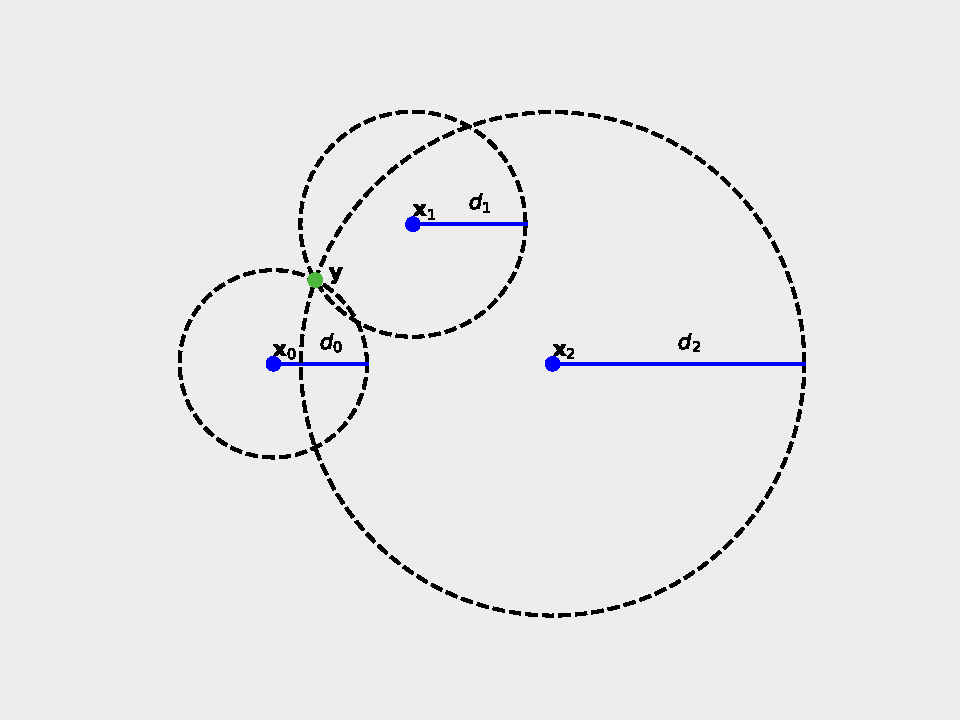
\includegraphics[width=.7\textwidth]{figs/trilateration_example.pdf}
  \caption{Position, $\mathbf{y}$, of entity determined by trilateration using known positions of $n = 3$ beacons.}
  \label[fig]{trilat_example}
\end{figure}
\todo{mention how spread of agents is benefitial and motivate it using litterature}

\subsection{Coverage}\label[secc]{coverage}
It is clear from subsection \ref{trilat} that three or more agents are needed to perform the task of multilateration. Hence a point $\mathbf{y}\in\mathcal{F}$ is said
to be \textit{covered} iff. it is within communication range of at least three agents, i.e. it is possible to determine the position of an entity placed at $\mathbf{y}$ through multilateration.

As discussed in subsection \ref{trilat} it is beneficial that agents used for multilateration spread out to some extent in order to ensure sufficient accuracy of multilateration.

\subsection{Constraints}\label[secc]{constraints}
It is clear from subsection \ref{trilat} that agents used as beacons in a multilateration scheme cannot be positioned on a straight line, as this would make it impossible
to uniquely determine the unknown position of an entity. Due to the fact that only agents close to the entity whose position is to be determined will
take part in the multilateration scheme, we impose only that agents that together can be used for multulateration must satisfy the non-linear position requirement in \eqref{nonlin_position}.

We also impose that any two agents must be some minimum distance apart at any given time. This is due to the fact that agents colliding could cause damage to the hardware, and possibly render them unusable.

\subsection{Objective function derivation}\label[secc]{obj_formulation}
The objective function presented here is inspired by \cite{sun2014escaping}, but differs in that for the purpose of multilateration, it is required that at least three agents must be within
range of a point in order for the point to be covered.

We assume we have a total of $N$ agents in a swarm $\mathcal{N}$ at our disposal. Furthermore we assume that all agents have the same maximum radius of communication:
\begin{equation}\label[eq]{homogenous_r}
  \begin{split}
    r_{a} &= r\;\forall\; a\in\mathcal{N}\\
  \end{split}
\end{equation}
Using \eqref{more_than_n_prob} we can express the probability of a point $\mathbf{y}$ being covered by the swarm as:
\begin{equation}\label[eq]{cover_prob}
  \Phi^{3^{+}}(\mathbf{X}_{\mathcal{N}}, \mathbf{y}) = 1 - \Phi^{0}(\mathbf{X}_{\mathcal{N}}, \mathbf{y}) - \Phi^{1}(\mathbf{X}_{\mathcal{N}}, \mathbf{y}) - \Phi^{2}(\mathbf{X}_{\mathcal{N}}, \mathbf{y})
\end{equation}
In order to formulate a distributed optimization algorithm, we rewrite the probability of coverage in \eqref{cover_prob} with focus on a single drone $a$.
We partition the swarm, $\mathcal{N}$, into two disjoint sets: $\{a\}$ and $\mathcal{N}\setminus\{a\}$. Using this we can rewrite \eqref{cover_prob} as:
\begin{equation}\label[eq]{distr_cover_derivation}
  \begin{split}
    \Phi^{3^{+}}(\mathbf{X}_{\mathcal{N}}, \mathbf{y}) &= 1\\
    &- \big(1-\hat{p}(\mathbf{x}_{a}, \mathbf{y})\big)\prod_{k\in\mathcal{N}\setminus\{a\}}\big(1-\hat{p}(\mathbf{x}_{k}, \mathbf{y}))\\
    &- \hat{p}(\mathbf{x}_{a}, \mathbf{y})\prod_{k\in\mathcal{N}\setminus\{a\}}\big(1-\hat{p}(\mathbf{x}_{k}, \mathbf{y}))\\
    &- \big(1-\hat{p}(\mathbf{x}_{a}, \mathbf{y})\big)\sum_{j\in\mathcal{N}\setminus\{a\}}\hat{p}(\mathbf{x}_{j}, \mathbf{y})\prod_{k\in\mathcal{N}\setminus\{a\}\setminus\{j\}}\big(1-\hat{p}(\mathbf{x}_{k}, \mathbf{y})\big)\\
    &- \hat{p}(\mathbf{x}_{a}, \mathbf{y})\sum_{j\in \mathcal{N}\setminus\{a\}}\hat{p}(\mathbf{x}_{j}, \mathbf{y})\prod_{k\in\mathcal{N}\setminus\{a\}\setminus\{j\}}\big(1-\hat{p}(\mathbf{x}_{k}, \mathbf{y})\big)\\
    &- \big(1-\hat{p}(\mathbf{x}_{a}, \mathbf{y})\big)\sum_{\mathcal{A}\in Comb(\mathcal{N}\setminus\{a\}, 2)}\prod_{j\in\mathcal{A}}\hat{p}(\mathbf{x}_{j}, \mathbf{y})\prod_{k\in\mathcal{N}\setminus\{a\}\setminus\mathcal{A}}\big(1-\hat{p}(\mathbf{x}_{k}, \mathbf{y})\big)\\
    &= 1\\
    &- \prod_{k\in\mathcal{N}\setminus\{a\}}\big(1-\hat{p}(\mathbf{x}_{k}, \mathbf{y}))\\
    &- \sum_{j\in\mathcal{N}\setminus\{a\}}\hat{p}(\mathbf{x}_{j}, \mathbf{y})\prod_{k\in\mathcal{N}\setminus\{a\}\setminus\{j\}}\big(1-\hat{p}(\mathbf{x}_{k}, \mathbf{y})\big)\\
    &- \big(1-\hat{p}(\mathbf{x}_{a}, \mathbf{y})\big)\sum_{\mathcal{A}\in Comb(\mathcal{N}\setminus\{a\}, 2)}\prod_{j\in\mathcal{A}}\hat{p}(\mathbf{x}_{j}, \mathbf{y})\prod_{k\in\mathcal{N}\setminus\{a\}\setminus\mathcal{A}}\big(1-\hat{p}(\mathbf{x}_{k}, \mathbf{y})\big)\\
  \end{split}
\end{equation}
Applying \eqref{Phi_def} to \eqref{distr_cover_derivation} yields:
\begin{equation}\label[eq]{local_coverage}
  \begin{split}
    \Phi^{3^{+}}(\mathbf{X}_{\mathcal{N}}, \mathbf{y}) &= 1 - \Phi^{0}(\mathbf{X}_{\mathcal{N}\setminus\{a\}}, \mathbf{y}) - \Phi^{1}(\mathbf{X}_{\mathcal{N}\setminus\{a\}}, \mathbf{y}) - \Phi^{2}(\mathbf{X}_{\mathcal{N}\setminus\{a\}}, \mathbf{y})\big(1-\hat{p}(\mathbf{x}_{a}, \mathbf{y})\big)\\
    &= \Phi^{3^{+}}(\mathbf{X}_{\mathcal{N}\setminus\{a\}}, \mathbf{y}) + \Phi^{2}(\mathbf{X}_{\mathcal{N}\setminus\{a\}}, \mathbf{y})\hat{p}(\mathbf{x}_{a}, \mathbf{y})\\
  \end{split}
\end{equation}
Rewriting \eqref{local_coverage} yields:
\begin{equation}
  \begin{split}
    \Phi^{3^{+}}(\mathbf{X}_{\mathcal{N}}, \mathbf{y}) &= \Phi^{3^{+}}(\mathbf{X}_{\mathcal{N}\setminus\{a\}}, \mathbf{y}) - \hat{p}(\mathbf{x}_{a}, \mathbf{y})\Phi^{3^{+}}(\mathbf{X}_{\mathcal{N}\setminus\{a\}}, \mathbf{y}) + \hat{p}(\mathbf{x}_{a}, \mathbf{y})\Phi^{2^{+}}(\mathbf{X}_{\mathcal{N}\setminus\{a\}}, \mathbf{y})\\
    &= (1-\hat{p}(\mathbf{x}_{a}, \mathbf{y}))\Phi^{3^{+}}(\mathbf{X}_{\mathcal{N}\setminus\{a\}}, \mathbf{y}) + \hat{p}(\mathbf{x}_{a}, \mathbf{y})\Phi^{2^{+}}(\mathbf{X}_{\mathcal{N}\setminus\{a\}}, \mathbf{y})\\
  \end{split}
\end{equation}
It is clear that the probability of the point $\mathbf{y}$ being covered can be seen on as an interpolation between two probability measures with the local probability of agent $a$ as the interpolation variable. Low local probability of agent $a$ means that the probability of coverage supplied the swarm as a whole depends more on the coverage supplied by
the swarm excluding agent $a$. In the extreme case where the local probability of agent $a$ is zero, the probability of covering $\mathbf{y}$ depends only on the coverage supplied by the swarm excluding agent $a$.

Higher local probability of agent $a$ means that the contribution of $a$ towards covering the point $\mathbf{y}$ is greater, thus less weight is put on the the probability of the swarm excluding agent $a$ covering the point. Instead more weight is put on the probability of at least \textit{two} other agents being able to communicate with an entity at $\mathbf{y}$. 
This is due to the fact that the probability of agent $a$ being able to communicate with said entity is higher, and we need only two or more other agents to be able to communicate with the entity at $\mathbf{y}$ to make the total number of agents covering $\mathbf{y}$ three or more.

\begin{figure}[H]
  \centering
  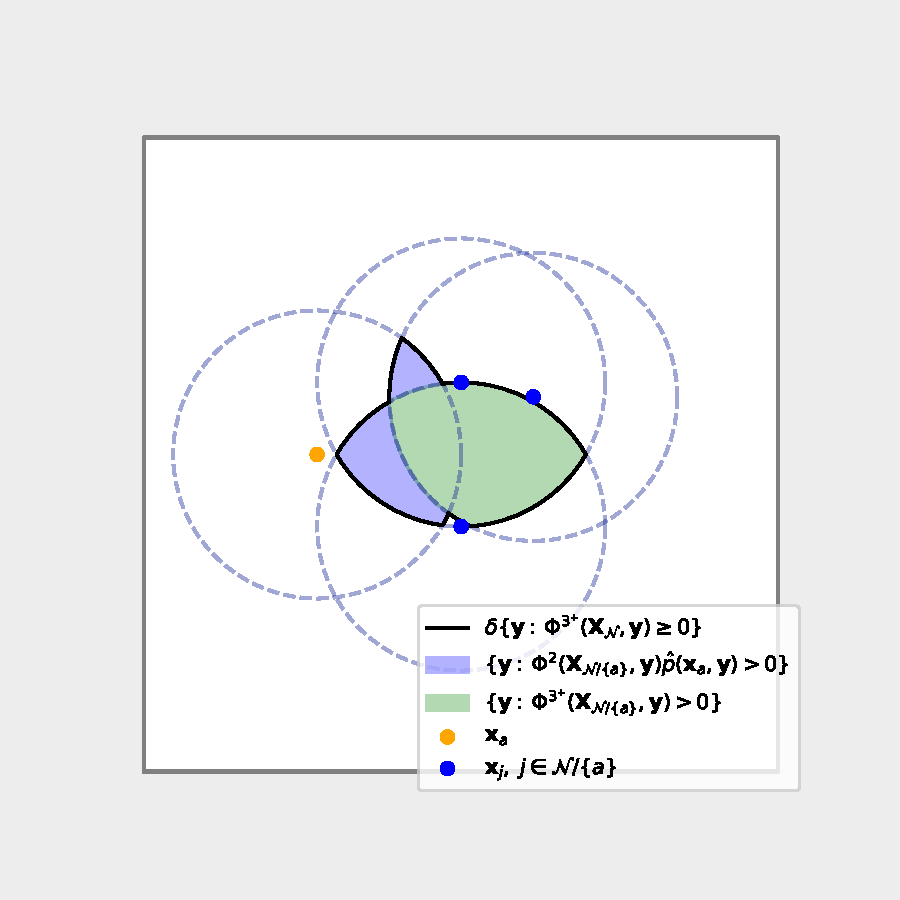
\includegraphics[width=.75\textwidth]{figs/local_objective_example.pdf}
  \caption{Non-zero regions of integrads in \eqref{rewritten_objective}. Note that perturbing the orange circle (position of agent $a$) does not affect the green region,
  as it is defined only by the intersections of the disks surrounding the blue points (other agents in the swarm).}
  \label[fig]{local_coverage_example}
\end{figure}

We note that the overall probability of coverage over the feasible space can be written as:
\begin{equation}\label[eq]{rewritten_objective}
  \begin{split}
    P(\mathbf{X}_{\mathcal{N}}) &=\int_{\mathcal{F}}\Phi^{3^{+}}(\mathbf{X}_{\mathcal{N}}, \mathbf{y})d\mathbf{y} =  \int_{\mathcal{F}}\Phi^{3^{+}}(\mathbf{X}_{\mathcal{N}\setminus\{a\}}, \mathbf{y}) + \Phi^{2}(\mathbf{X}_{\mathcal{N}\setminus\{a\}}, \mathbf{y})\hat{p}(\mathbf{x}_{a}, \mathbf{y})d\mathbf{y}\\
    &= \int_{\mathcal{F}}\Phi^{3^{+}}(\mathbf{X}_{\mathcal{N}\setminus\{a\}}, \mathbf{y})d\mathbf{y} + \int_{\mathcal{F}}\Phi^{2}(\mathbf{X}_{\mathcal{N}\setminus\{a\}}, \mathbf{y})\hat{p}(\mathbf{x}_{a}, \mathbf{y})d\mathbf{y}\\
  \end{split}
\end{equation}
We note that the first term in \eqref{rewritten_objective} is independent of the position of $a$ in both its domain and integrand. This independence is visualized in \figref{local_coverage_example}. Thus we can rewrite the overall coverage probability over $\mathcal{F}$ as:
\begin{equation}
  P(\mathbf{X}_{\mathcal{N}}) = P(\mathbf{X}_{\mathcal{N}\setminus\{a\}}) + P_{a}(\mathbf{X}_{\mathcal{N}})
\end{equation}
Where the \textit{local} probability of coverage for agent $a$ over the feasible space is defined as:
\begin{equation}\label[eq]{local_objective}
  P_{a}(\mathbf{X}_{\mathcal{N}}) = \int_{\mathcal{F}}\Phi^{2}(\mathbf{X}_{\mathcal{N}\setminus\{a\}}, \mathbf{y})\hat{p}(\mathbf{x}_{a}, \mathbf{y})d\mathbf{y}
\end{equation}

As in \cite{sun2014escaping} we note that from the viewpoint of agent $a$, the swarm can be partitioned into three disjoint sets: $\{a\}$, $\mathcal{B}_{a}$ and $\mathcal{C}_{a}$. The latter sets are defined as:
\begin{subequations}\label[eq]{neigh_def}
  \begin{equation}
    \mathcal{B}_{a} = \{j\in\mathcal{N}\setminus\{a\}: \norm{\mathbf{x}_{a}-\mathbf{x}_{j}} \leq 2r\}
  \end{equation}
  \begin{equation}
    \mathcal{C}_{a} = \{j\in\mathcal{N}\setminus\{a\}: \norm{\mathbf{x}_{a}-\mathbf{x}_{j}} > 2r\}
  \end{equation}  
\end{subequations}
The set $\mathcal{B}_{a}$, from now on called the neighbours of $a$, contains all agents in the swarm, $\mathcal{N}$, whose communication disks form a non-empty intersection with that of $a$.
$\mathcal{C}_{a}$ contains all agents whose communication disks do not intersect with that of $a$.

Applying \eqref{neigh_def} to \eqref{local_objective} yields:
\begin{equation}
  \begin{split}
    P_{a}(\mathbf{X}_{\mathcal{N}}) &= \int_{\mathcal{F}}\Phi^{2}(\mathbf{X}_{\mathcal{N}\setminus\{a\}}, \mathbf{y})\hat{p}(\mathbf{x}_{a}, \mathbf{y})d\mathbf{y}\\
    &= \int_{\mathcal{F}}\Big(\Phi^{2}(\mathbf{X}_{\mathcal{B}_{a}}, \mathbf{y}) + \Phi^{2}(\mathbf{X}_{\mathcal{C}_{a}}, \mathbf{y}) + \Phi^{1}(\mathbf{X}_{\mathcal{B}_{a}}, \mathbf{y})\Phi^{1}(\mathbf{X}_{\mathcal{C}_{a}}, \mathbf{y})\Big)\hat{p}(\mathbf{x}_{a}, \mathbf{y})d\mathbf{y}
  \end{split}
\end{equation}
Partitioning the domain of integration into the visible set and invisible set of agent $a$, and noting that $\hat{p}(\mathbf{x}_{j}, \mathbf{y}) = 0\;\forall\;j\in\mathcal{C}_{a},\;\mathbf{y}\in V_{a}$ such that
$\Phi^{n}(\mathbf{X}_{\mathcal{C}_{a}}, \mathbf{y}) = 0\;\forall\;n\in\mathbb{Z}^{+},\;\mathbf{y}\in V_{a}$, and $\hat{p}(\mathbf{x}_{a}, \mathbf{y}) = 0\;\forall\;\mathbf{y}\in U_{a}$ yields:
\begin{equation}\label[eq]{local_objective_derivated}
  \begin{split}
    P_{a}(\mathbf{X}_{\mathcal{N}}) &= \int_{V_{a}}\Big(\Phi^{2}(\mathbf{X}_{\mathcal{B}_{a}}, \mathbf{y}) + \Phi^{2}(\mathbf{X}_{\mathcal{C}_{a}}, \mathbf{y}) + \Phi^{1}(\mathbf{X}_{\mathcal{B}_{a}}, \mathbf{y})\Phi^{1}(\mathbf{X}_{\mathcal{C}_{a}}, \mathbf{y})\Big)\hat{p}(\mathbf{x}_{a}, \mathbf{y})d\mathbf{y}\\
    &+ \int_{U_{a}}\Big(\Phi^{2}(\mathbf{X}_{\mathcal{B}_{a}}, \mathbf{y}) + \Phi^{2}(\mathbf{X}_{\mathcal{C}_{a}}, \mathbf{y}) + \Phi^{1}(\mathbf{X}_{\mathcal{B}_{a}}, \mathbf{y})\Phi^{1}(\mathbf{X}_{\mathcal{C}_{a}}, \mathbf{y})\Big)\hat{p}(\mathbf{x}_{a}, \mathbf{y})d\mathbf{y}\\
    &= \int_{V_{a}}\Phi^{2}(\mathbf{X}_{\mathcal{B}_{a}}, \mathbf{y})p(\norm{\mathbf{x}_{a}-\mathbf{y}})d\mathbf{y} = L(\mathbf{X}_{\mathcal{B}_{a}\cup\{a\}})
  \end{split}
\end{equation}
Thus the local probability of coverage for an agent $a$ is dependent on the position, $\mathbf{x}_{a}$, of agent $a$ in both domain and integrand, and the positions of the neighbours of agent $a$.
We call the swarm consisting of $a$ and its neighbours agent $a$'s local swarm.

We measure the proximity of two agents, $a$ and $j$, by:
\begin{equation}\label[eq]{proximity_func}
  D(\mathbf{x}_{a}, \mathbf{x}_{j}) = k_{1}e^{-k_{2}\norm{\mathbf{x}_{a} - \mathbf{x}_{j}}}
\end{equation}
The function has two tunable parameters, $k_{1}$ and $k_{2}$, whose effect is show in \figref{cdr}.

Using \eqref{local_objective_derivated} and \eqref{proximity_func}  We now state the \textit{local} objective for an agent $a$ as:
\begin{equation}\label[eq]{local_objective_func}
  H(\mathbf{X}_{\mathcal{B}_{a}\cup\{a\}})  = L(\mathbf{X}_{\mathcal{B}_{a}\cup\{a\}})  - \sum_{j\in\mathcal{B}_{a}}D(\mathbf{x}_{a}, \mathbf{x}_{j})
\end{equation}
where the second term is added to ensure sufficient spread of agents.
\begin{figure}[H]
  \centering
  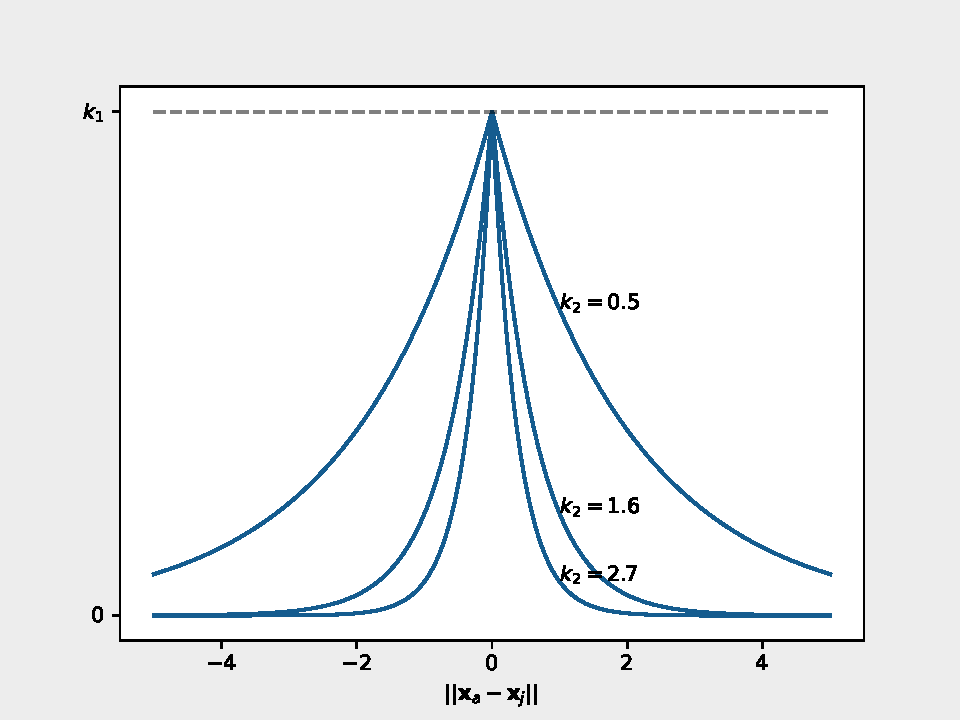
\includegraphics[width=.7\textwidth]{figs/close_dist_repell_example.pdf}
  \caption{Proximity term in \eqref{totally_objective} for two agents.}
  \label[fig]{cdr}
\end{figure}

\subsection{Optimization problem formulation}
Using \eqref{local_objective_func} and the constraints mentioned in \ref{constraints}, we define the optimization problem as:
\begin{equation}\label[eq]{totally_objective}
  \begin{split}
    \max_{\mathbf{x}_{a}}&\;H(\mathbf{X}_{\mathcal{B}_{a}\cup\{a\}}) \\
    \mathrm{s.t.}\;&\mathbf{x}_{a}\in\mathcal{F}\\
    & |\mathcal{B}_{a}|\geq 2\\
    \norm{\mathbf{x}_{a} - \mathbf{x}_{j}} &\geq r_{min}\;\forall\;j\in\mathcal{B}_{a}\\
    \mathrm{Rank(\mathbf{V})} &= 2\\
    \mathbf{V} &= \begin{bmatrix}
      \mathbf{x}_{a} - \mathbf{X}_{\mathcal{B}_{a}, 0}&\hdots&\mathbf{x}_{a}-\mathbf{X}_{\mathcal{B}_{a}, |B_{a}|-1}
    \end{bmatrix}\\
  \end{split}
\end{equation}
The second term of the objective in \eqref{totally_objective} penalizes the clustering of agents. In essence it works
as anti-gravity between neighbours, as it will cause agent $a$ to move away from it's neighbouring agents.

The equality constraints in \eqref{totally_objective} impose that agent $a$ is not placed such that it lies on a straight line through all it's neighbours. Furthermore they implicitly impose that agent $a$ has at least two 
neighbours at all times, as $\mathrm{Rank}(\mathbf{V}) \leq \min(n, m)$ for a matrix $\mathbf{V}\in\mathbb{R}^{n\times m}$.
